% Options for packages loaded elsewhere
\PassOptionsToPackage{unicode}{hyperref}
\PassOptionsToPackage{hyphens}{url}
%
\documentclass[
]{article}
\usepackage{amsmath,amssymb}
\usepackage{iftex}
\ifPDFTeX
  \usepackage[T1]{fontenc}
  \usepackage[utf8]{inputenc}
  \usepackage{textcomp} % provide euro and other symbols
\else % if luatex or xetex
  \usepackage{unicode-math} % this also loads fontspec
  \defaultfontfeatures{Scale=MatchLowercase}
  \defaultfontfeatures[\rmfamily]{Ligatures=TeX,Scale=1}
\fi
\usepackage{xcoffins}
\usepackage{lmodern}

\ifPDFTeX\else
% xetex/luatex font selection
    \setmainfont[]{David}
\fi
% Use upquote if available, for straight quotes in verbatim environments
\IfFileExists{upquote.sty}{\usepackage{upquote}}{}
\IfFileExists{microtype.sty}{% use microtype if available
  \usepackage[]{microtype}
  \UseMicrotypeSet[protrusion]{basicmath} % disable protrusion for tt fonts
}{}
\makeatletter
\@ifundefined{KOMAClassName}{% if non-KOMA class
  \IfFileExists{parskip.sty}{%
    \usepackage{parskip}
  }{% else
    \setlength{\parindent}{0pt}
    \setlength{\parskip}{6pt plus 2pt minus 1pt}}
}{% if KOMA class
  \KOMAoptions{parskip=half}}
\makeatother
\usepackage{xcolor}
\usepackage{fancyvrb}
\newcommand{\VerbBar}{|}
\newcommand{\VERB}{\Verb[commandchars=\\\{\}]}
\DefineVerbatimEnvironment{Highlighting}{Verbatim}{commandchars=\\\{\}}
% Add ',fontsize=\small' for more characters per line
\newenvironment{Shaded}{}{}
\newcommand{\AlertTok}[1]{\textcolor[rgb]{1.00,0.00,0.00}{\textbf{#1}}}
\newcommand{\AnnotationTok}[1]{\textcolor[rgb]{0.38,0.63,0.69}{\textbf{\textit{#1}}}}
\newcommand{\AttributeTok}[1]{\textcolor[rgb]{0.49,0.56,0.16}{#1}}
\newcommand{\BaseNTok}[1]{\textcolor[rgb]{0.25,0.63,0.44}{#1}}
\newcommand{\BuiltInTok}[1]{\textcolor[rgb]{0.00,0.50,0.00}{#1}}
\newcommand{\CharTok}[1]{\textcolor[rgb]{0.25,0.44,0.63}{#1}}
\newcommand{\CommentTok}[1]{\textcolor[rgb]{0.38,0.63,0.69}{\textit{#1}}}
\newcommand{\CommentVarTok}[1]{\textcolor[rgb]{0.38,0.63,0.69}{\textbf{\textit{#1}}}}
\newcommand{\ConstantTok}[1]{\textcolor[rgb]{0.53,0.00,0.00}{#1}}
\newcommand{\ControlFlowTok}[1]{\textcolor[rgb]{0.00,0.44,0.13}{\textbf{#1}}}
\newcommand{\DataTypeTok}[1]{\textcolor[rgb]{0.56,0.13,0.00}{#1}}
\newcommand{\DecValTok}[1]{\textcolor[rgb]{0.25,0.63,0.44}{#1}}
\newcommand{\DocumentationTok}[1]{\textcolor[rgb]{0.73,0.13,0.13}{\textit{#1}}}
\newcommand{\ErrorTok}[1]{\textcolor[rgb]{1.00,0.00,0.00}{\textbf{#1}}}
\newcommand{\ExtensionTok}[1]{#1}
\newcommand{\FloatTok}[1]{\textcolor[rgb]{0.25,0.63,0.44}{#1}}
\newcommand{\FunctionTok}[1]{\textcolor[rgb]{0.02,0.16,0.49}{#1}}
\newcommand{\ImportTok}[1]{\textcolor[rgb]{0.00,0.50,0.00}{\textbf{#1}}}
\newcommand{\InformationTok}[1]{\textcolor[rgb]{0.38,0.63,0.69}{\textbf{\textit{#1}}}}
\newcommand{\KeywordTok}[1]{\textcolor[rgb]{0.00,0.44,0.13}{\textbf{#1}}}
\newcommand{\NormalTok}[1]{#1}
\newcommand{\OperatorTok}[1]{\textcolor[rgb]{0.40,0.40,0.40}{#1}}
\newcommand{\OtherTok}[1]{\textcolor[rgb]{0.00,0.44,0.13}{#1}}
\newcommand{\PreprocessorTok}[1]{\textcolor[rgb]{0.74,0.48,0.00}{#1}}
\newcommand{\RegionMarkerTok}[1]{#1}
\newcommand{\SpecialCharTok}[1]{\textcolor[rgb]{0.25,0.44,0.63}{#1}}
\newcommand{\SpecialStringTok}[1]{\textcolor[rgb]{0.73,0.40,0.53}{#1}}
\newcommand{\StringTok}[1]{\textcolor[rgb]{0.25,0.44,0.63}{#1}}
\newcommand{\VariableTok}[1]{\textcolor[rgb]{0.10,0.09,0.49}{#1}}
\newcommand{\VerbatimStringTok}[1]{\textcolor[rgb]{0.25,0.44,0.63}{#1}}
\newcommand{\WarningTok}[1]{\textcolor[rgb]{0.38,0.63,0.69}{\textbf{\textit{#1}}}}
\usepackage{longtable,booktabs,array}
\usepackage{calc} % for calculating minipage widths
% Correct order of tables after \paragraph or \subparagraph
\usepackage{etoolbox}
\makeatletter
\patchcmd\longtable{\par}{\if@noskipsec\mbox{}\fi\par}{}{}
\makeatother
% Allow footnotes in longtable head/foot
\IfFileExists{footnotehyper.sty}{\usepackage{footnotehyper}}{\usepackage{footnote}}
\makesavenoteenv{longtable}
\usepackage{graphicx}
\makeatletter
\def\maxwidth{\ifdim\Gin@nat@width>\linewidth\linewidth\else\Gin@nat@width\fi}
\def\maxheight{\ifdim\Gin@nat@height>\textheight\textheight\else\Gin@nat@height\fi}
\makeatother
% Scale images if necessary, so that they will not overflow the page
% margins by default, and it is still possible to overwrite the defaults
% using explicit options in \includegraphics[width, height, ...]{}
\setkeys{Gin}{width=\maxwidth,height=\maxheight,keepaspectratio}
% Set default figure placement to htbp
\makeatletter
\def\fps@figure{htbp}
\makeatother
\setlength{\emergencystretch}{3em} % prevent overfull lines
\providecommand{\tightlist}{%
  \setlength{\itemsep}{0pt}\setlength{\parskip}{0pt}}
\setcounter{secnumdepth}{-\maxdimen} % remove section numbering
\ifLuaTeX
\usepackage[bidi=basic]{babel}
\else
\usepackage[bidi=default]{babel}
\fi
\babelprovide[main,import]{hebrew}
\ifPDFTeX
\else
\babelfont{rm}[]{David}
\fi
% get rid of language-specific shorthands (see #6817):
\let\LanguageShortHands\languageshorthands
\def\languageshorthands#1{}
\ifLuaTeX
  \usepackage{selnolig}  % disable illegal ligatures
\fi
\ifPDFTeX
  \TeXXeTstate=1
  \newcommand{\RL}[1]{\beginR #1\endR}
  \newcommand{\LR}[1]{\beginL #1\endL}
  \newenvironment{RTL}{\beginR}{\endR}
  \newenvironment{LTR}{\beginL}{\endL}
\fi
\usepackage{bookmark}
\IfFileExists{xurl.sty}{\usepackage{xurl}}{} % add URL line breaks if available
\urlstyle{same}
\hypersetup{
  pdflang={he},
  hidelinks,
  pdfcreator={LaTeX via pandoc}}

\usepackage{bidi}


\author{}
\date{}

\begin{document}
\setRTL

\NewCoffin\Output   %Coffin to hold the others 
\NewCoffin\Callout % Callout definition ...
\NewCoffin\BackFrame % Background: green rectangle
\NewCoffin\SideRule  %lateral left border


\newcommand{\SetCallout}[2]{%
    \SetHorizontalCoffin\Output{} % It will be the reference point join the others  
    \SetVerticalCoffin\Callout{\linewidth}{\textbf{#1} #2}

    %% Make both \BackFrame & SideRule heights = height of Callout + 1*baselineskip
    \SetHorizontalCoffin\BackFrame{\color{green!30!gray!15}\rule{\linewidth}{\CoffinTotalHeight\Callout + \baselineskip}} 
    \SetHorizontalCoffin\SideRule{\textcolor{green}{\rule{3pt}{\CoffinTotalHeight\Callout +\baselineskip}}} %vertical side rule 

    %% Assembly Coffins
    \JoinCoffins*\Output[l,t]\BackFrame[l,t] %attach left-top corner of BackFrame  to idem of Output
    \JoinCoffins*\Output[l,t]\SideRule[l,t] %attach left-top corner of  SideRule to idem of Output
    \JoinCoffins*\Output[l,t]\Callout[l,t](0pt,-\baselineskip) %attach left-top corner of Callout to idem of Output
    %% Typeset ooutput
    \noindent\TypesetCoffin\Output % at the text insertion point. It is not a float.
    \vspace*{\CoffinTotalHeight\Callout}\bigskip %make some room for Output
}

\begin{longtable}[]{@{}ll@{}}
\toprule\noalign{}
& סטודנט א' \\
\midrule\noalign{}
\endhead
\bottomrule\noalign{}
\endlastfoot
\textbf{שם} & עידו פנג בנטוב \\
\textbf{ת''ז} & 322869140 \\
\textbf{דואר אלקטרוני} & ido.fang@campus.technion.ac.il \\
\end{longtable}

{\color{green!30!gray!15} \rule{10pt}{1pt}}

\begin{longtable}[]{@{}ll@{}}
\toprule\noalign{}
& סטודנט ב' \\
\midrule\noalign{}
\endhead
\bottomrule\noalign{}
\endlastfoot
\textbf{שם} & ניר קרל \\
\textbf{ת''ז} & 322437203 \\
\textbf{דואר אלקטרוני} & nir.karl@campus.technion.ac.il \\
\end{longtable}

\subsection{תרגיל 1}\label{ux5eaux5e8ux5d2ux5d9ux5dc-1}

\subsubsection{סעיף א'}\label{ux5e1ux5e2ux5d9ux5e3-ux5d0}

הקוד הכולל של סעיף א' וסעיף ב' ב-\texttt{python}:

\begin{Shaded}
\begin{Highlighting}[]
\ImportTok{import}\NormalTok{ numpy }\ImportTok{as}\NormalTok{ np}
\ImportTok{import}\NormalTok{ matplotlib.pyplot }\ImportTok{as}\NormalTok{ plt}

\KeywordTok{def}\NormalTok{ weight(j, point\_x):}
\NormalTok{    w }\OperatorTok{=} \DecValTok{1}
\NormalTok{    n }\OperatorTok{=} \BuiltInTok{len}\NormalTok{(point\_x)}
    \ControlFlowTok{for}\NormalTok{ i }\KeywordTok{in} \BuiltInTok{range}\NormalTok{(n):}
        \ControlFlowTok{if}\NormalTok{ i }\OperatorTok{!=}\NormalTok{ j:}
\NormalTok{            w }\OperatorTok{*=}\NormalTok{ (}\DecValTok{1} \OperatorTok{/}\NormalTok{ (point\_x[j] }\OperatorTok{{-}}\NormalTok{ point\_x[i]))}
    \ControlFlowTok{return}\NormalTok{ w}

\KeywordTok{def}\NormalTok{ helper\_polynom(x, point\_x):}
\NormalTok{    phi }\OperatorTok{=} \DecValTok{1}
\NormalTok{    n }\OperatorTok{=} \BuiltInTok{len}\NormalTok{(point\_x)}
    \ControlFlowTok{for}\NormalTok{ i }\KeywordTok{in} \BuiltInTok{range}\NormalTok{(n):}
\NormalTok{        phi }\OperatorTok{*=}\NormalTok{ (x }\OperatorTok{{-}}\NormalTok{ point\_x[i])}
    \ControlFlowTok{return}\NormalTok{ phi}
\end{Highlighting}
\end{Shaded}

\begin{Shaded}
\begin{Highlighting}[]
    
\KeywordTok{def}\NormalTok{ lagrange(f, n, a, b):}
\NormalTok{    point\_x }\OperatorTok{=}\NormalTok{ np.linspace(a, b, n)}
\NormalTok{    point\_y }\OperatorTok{=}\NormalTok{ f(point\_x)}
\NormalTok{    w }\OperatorTok{=}\NormalTok{ [weight(j, point\_x) }\ControlFlowTok{for}\NormalTok{ j }\KeywordTok{in} \BuiltInTok{range}\NormalTok{(n)]}
    
    \CommentTok{\# Evaluate p at 0.01 intervals}
\NormalTok{    t }\OperatorTok{=} \FloatTok{0.01}
\NormalTok{    x }\OperatorTok{=}\NormalTok{ np.linspace(a, b, }\BuiltInTok{int}\NormalTok{((b }\OperatorTok{{-}}\NormalTok{ a) }\OperatorTok{/}\NormalTok{ t) }\OperatorTok{+} \DecValTok{1}\NormalTok{)}
\NormalTok{    p }\OperatorTok{=}\NormalTok{ np.zeros\_like(x)}
\NormalTok{    phi }\OperatorTok{=}\NormalTok{ np.zeros\_like(x)}
    \ControlFlowTok{for}\NormalTok{ k }\KeywordTok{in} \BuiltInTok{range}\NormalTok{(}\BuiltInTok{len}\NormalTok{(x)):}
        \ControlFlowTok{for}\NormalTok{ j }\KeywordTok{in} \BuiltInTok{range}\NormalTok{(n):}
\NormalTok{            p[k] }\OperatorTok{+=}\NormalTok{ (w[j] }\OperatorTok{*}\NormalTok{ point\_y[j]) }\OperatorTok{/}\NormalTok{ (x[k] }\OperatorTok{{-}}\NormalTok{ point\_x[j])}
\NormalTok{        phi[k] }\OperatorTok{=}\NormalTok{ helper\_polynom(x[k], point\_x)}
\NormalTok{        p[k] }\OperatorTok{=}\NormalTok{ phi[k] }\OperatorTok{*}\NormalTok{ p[k]}
    \ControlFlowTok{return}\NormalTok{ x, p, phi}

\KeywordTok{def}\NormalTok{ f(x):}
    \ControlFlowTok{return}\NormalTok{ np.cos(}\DecValTok{2} \OperatorTok{*}\NormalTok{ np.pi }\OperatorTok{*}\NormalTok{ x)}

\NormalTok{a }\OperatorTok{=} \OperatorTok{{-}}\DecValTok{1}
\NormalTok{b }\OperatorTok{=} \DecValTok{1}
\NormalTok{n }\OperatorTok{=}\NormalTok{ [}\DecValTok{2}\NormalTok{, }\DecValTok{5}\NormalTok{, }\DecValTok{10}\NormalTok{, }\DecValTok{20}\NormalTok{]}

\CommentTok{\# n derivative of f}

\NormalTok{f\_n }\OperatorTok{=}\NormalTok{ [}
    \KeywordTok{lambda}\NormalTok{ x: }\OperatorTok{{-}}\NormalTok{((}\DecValTok{2} \OperatorTok{*}\NormalTok{ np.pi) }\OperatorTok{**} \DecValTok{2}\NormalTok{) }\OperatorTok{*}\NormalTok{ np.cos(}\DecValTok{2} \OperatorTok{*}\NormalTok{ np.pi }\OperatorTok{*}\NormalTok{ x),}
    \KeywordTok{lambda}\NormalTok{ x: }\OperatorTok{{-}}\NormalTok{((}\DecValTok{2} \OperatorTok{*}\NormalTok{ np.pi) }\OperatorTok{**} \DecValTok{5}\NormalTok{) }\OperatorTok{*}\NormalTok{ np.sin(}\DecValTok{2} \OperatorTok{*}\NormalTok{ np.pi }\OperatorTok{*}\NormalTok{ x),}
    \KeywordTok{lambda}\NormalTok{ x: }\OperatorTok{{-}}\NormalTok{((}\DecValTok{2} \OperatorTok{*}\NormalTok{ np.pi) }\OperatorTok{**} \DecValTok{10}\NormalTok{) }\OperatorTok{*}\NormalTok{ np.cos(}\DecValTok{2} \OperatorTok{*}\NormalTok{ np.pi }\OperatorTok{*}\NormalTok{ x),}
    \KeywordTok{lambda}\NormalTok{ x: ((}\DecValTok{2} \OperatorTok{*}\NormalTok{ np.pi) }\OperatorTok{**} \DecValTok{20}\NormalTok{) }\OperatorTok{*}\NormalTok{ np.cos(}\DecValTok{2} \OperatorTok{*}\NormalTok{ np.pi }\OperatorTok{*}\NormalTok{ x)}
\NormalTok{]}

\NormalTok{graph\_i }\OperatorTok{=}\NormalTok{ plt.figure()}
\NormalTok{plt.title(}\StringTok{"Interpolant evaluations"}\NormalTok{)}
\NormalTok{plt.plot(np.linspace(a, b, }\DecValTok{100}\NormalTok{), f(np.linspace(a, b, }\DecValTok{100}\NormalTok{)))}
\end{Highlighting}
\end{Shaded}

\begin{Shaded}
\begin{Highlighting}[]

\ControlFlowTok{for}\NormalTok{ k }\KeywordTok{in} \BuiltInTok{range}\NormalTok{(}\BuiltInTok{len}\NormalTok{(n)):}
    \CommentTok{\# Interpolant evaluation}
\NormalTok{    plt.figure(graph\_i.number)}
    
\NormalTok{    x, p, phi }\OperatorTok{=}\NormalTok{ lagrange(f, n[k], a, b)}
\NormalTok{    plt.plot(x, p, }\StringTok{"{-}{-}"}\NormalTok{)}
    
    \CommentTok{\# Absolute error}
\NormalTok{    graph\_e }\OperatorTok{=}\NormalTok{ plt.figure()}
\NormalTok{    plt.title(}\StringTok{"n = "} \OperatorTok{+} \BuiltInTok{str}\NormalTok{(n[k]) }\OperatorTok{+} \StringTok{" error"}\NormalTok{)}
    
\NormalTok{    fval }\OperatorTok{=}\NormalTok{ f(x)}
\NormalTok{    e\_abs }\OperatorTok{=}\NormalTok{ np.}\BuiltInTok{abs}\NormalTok{(fval }\OperatorTok{{-}}\NormalTok{ p)}
\NormalTok{    plt.plot(x, e\_abs)}
    
    \CommentTok{\# Error boundaries}
\NormalTok{    fnxi }\OperatorTok{=}\NormalTok{ np.}\BuiltInTok{max}\NormalTok{(np.}\BuiltInTok{abs}\NormalTok{(f\_n[k](np.arange(}\OperatorTok{{-}}\DecValTok{1}\NormalTok{, }\FloatTok{1.25}\NormalTok{, }\FloatTok{0.25}\NormalTok{))))}
\NormalTok{    e\_boundary }\OperatorTok{=}\NormalTok{ np.}\BuiltInTok{abs}\NormalTok{(phi) }\OperatorTok{*}\NormalTok{ (fnxi }\OperatorTok{*}\NormalTok{ (}\DecValTok{1} \OperatorTok{/}\NormalTok{ np.math.factorial(n[k])))}

\NormalTok{    plt.plot(x, e\_boundary, }\StringTok{"{-}{-}"}\NormalTok{)}
\NormalTok{    plt.legend([}\StringTok{"Absolute error"}\NormalTok{, }\StringTok{"Error boundary"}\NormalTok{])}

\NormalTok{plt.figure(graph\_i.number)}
\NormalTok{plt.legend([}\StringTok{"f(x)"}\NormalTok{, }\StringTok{"n=2"}\NormalTok{, }\StringTok{"n=5"}\NormalTok{, }\StringTok{"n=10"}\NormalTok{, }\StringTok{"n=20"}\NormalTok{])}
\NormalTok{plt.show()}
\end{Highlighting}
\end{Shaded}

\begin{figure}
\centering
\beginR{\beginL{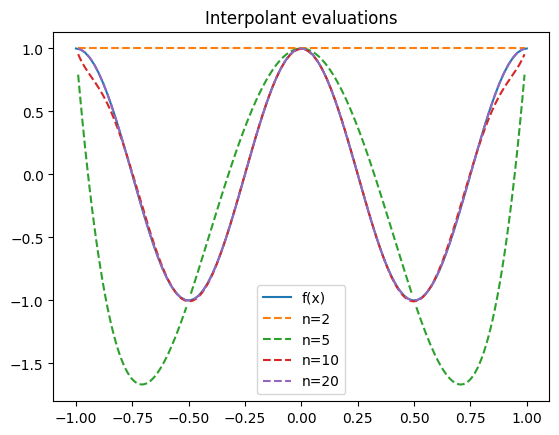
\includegraphics[width=\textwidth,height=0.4\textheight]{NUM1_HW005/evals.png}}}
\caption{book}
\end{figure}

\SetCallout{הערה:}{
של \(f(x)\) ו-\(p_{19}\) מאוד דומים, ולכן הם פשוט נמצאים בגרף אחד על
השני.
}

\subsubsection{סעיף ב'}\label{ux5e1ux5e2ux5d9ux5e3-ux5d1}

מאחר והנגזרות של \(f(x)\) הן כולן פונקציות של \(\cos(2\pi x)\) או
\(\sin(2\pi x)\) בכפולות שונות, ערכן המקסימלי תמיד יתקבל באחד מהערכים:
\[x=-1,-0.75,-0.5,\dots,\, 0.75,\, 1 \] ולכן מספיק לחשב את ערכי הנגזרת
רק בהן. ברור שעבור רוב הנקודות הערכים יהיו זהים, אבל זה רק מוסיף כמה
בדיקות בודדות, אז טוב לקחת מקדם ביטחון.

\SetCallout{
הערה:
}{
\(n\) שלנו בשאלה הוא שונה מה-\(n\) שנתונה בנוסחה (וזה למה הוגדר \(N\)
שונה מ-\(n\) בשאלה). לכן, בקוד, ה-\(n\) שאנו משתמשים בו לחישוב הוא
\(n-1\), כך שמקבלים את הנוסחה:
\[\left|e_{n}(x)\right|\leq \dfrac{1}{(n)!}\cdot\psi(x)\cdot \max_{\xi \in [-1,1]}\left|f^{(n)}(\xi)\right|\]
}

קיבלנו כי החסם לשגיאה אכן מהווה חסם לשגיאה האמיתית:

\begin{figure}
\centering
\beginR{\beginL{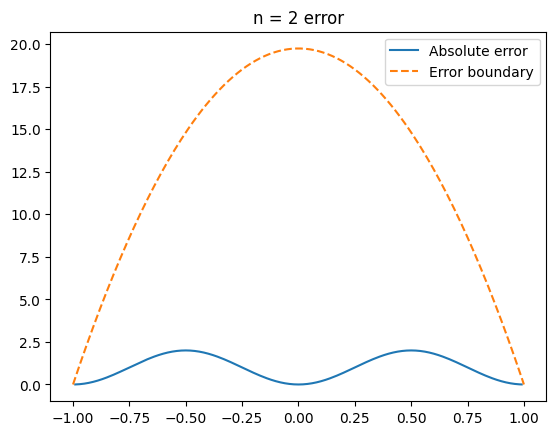
\includegraphics[width=\textwidth,height=0.4\textheight]{NUM1_HW005/n2.png}}}
\caption{book}
\end{figure}

\begin{figure}
\centering
\beginR{\beginL{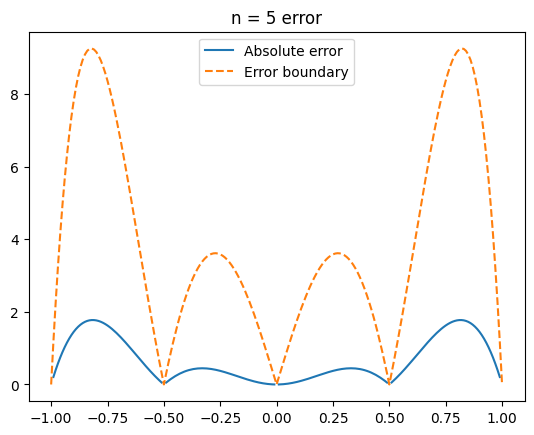
\includegraphics[width=\textwidth,height=0.4\textheight]{NUM1_HW005/n5.png}}}
\caption{book}
\end{figure}

\begin{figure}
\centering
\beginR{\beginL{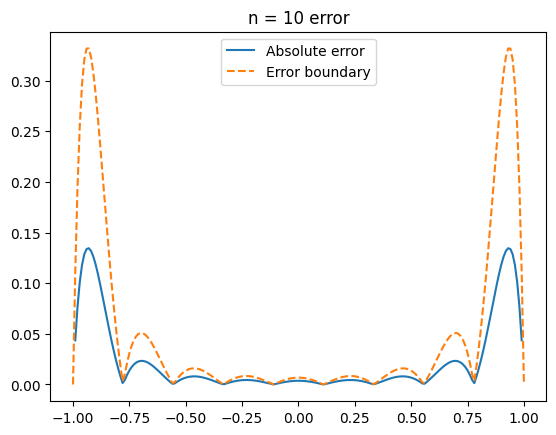
\includegraphics[width=\textwidth,height=0.4\textheight]{NUM1_HW005/n10.png}}}
\caption{book}
\end{figure}

\begin{figure}
\centering
\beginR{\beginL{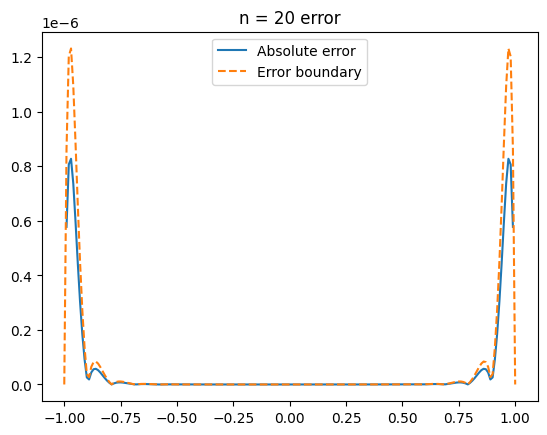
\includegraphics[width=\textwidth,height=0.4\textheight]{NUM1_HW005/n20.png}}}
\caption{book}
\end{figure}

\subsection{תרגיל 2}\label{ux5eaux5e8ux5d2ux5d9ux5dc-2}

\subsubsection{סעיף א'}\label{ux5e1ux5e2ux5d9ux5e3-ux5d0-1}

נחשב את פולינום הבסיס עבור כל אחד מה-\(x\) הנתונים:
\[L _{i}=\prod_{\begin{array}{c}
j=0 \\
i\neq j
\end{array}}^{2}=\frac{x-x_{j}}{x_{i}-x_{j}}\]

\[\begin{aligned}
&\begin{aligned}
L_{0}(x):& \\
 & j=0:\; i=j\Longrightarrow \emptyset \\
 & j=1:\; \frac{x-0}{-1-0}=-x \\
 & j=2:\; \frac{x-1}{-1-1}=-\frac{x}{2}+\frac{1}{2} \\
&L_{0}(x)=(-x)\cdot \left(- \frac{x}{2}+\frac{1}{2} \right)=\frac{x^{2}}{2}-\frac{x}{2}
\end{aligned}\\
&\begin{aligned}
L_{1}(x):& \\
&j=0:\; \frac{x-(-1)}{0-(-1)}=x+1 \\
&j=1:\;i=j\Longrightarrow \emptyset \\
&j=2:\; \frac{x-1}{0-1}=-x+1 \\
&L _{1(x)}=(x+1)(-x+1)=-x^{2}+1
\end{aligned}\\
&\begin{aligned}\\
L_{2}(x): \\
& j=0:\;\frac{x-(-1)}{1-(-1)}=\frac{x}{2}+\frac{1}{2} \\
& j=1:\;\frac{x-0}{1-0}=x \\
& j=2:\;i=j\Longrightarrow \emptyset \\
&L _{2}=\left( \frac{x}{2}+\frac{1}{2} \right)\cdot x=\frac{x^{2}}{2}+\frac{x}{2}
\end{aligned}\\
\end{aligned}\]

\subsubsection{סעיף ב'}\label{ux5e1ux5e2ux5d9ux5e3-ux5d1-1}

\[\sum_{i=0}^{2}L _{i}(x)=\left( \frac{x^{2}}{2}-\frac{x}{2} \right)+(-x^{2}+1)+\left( \frac{x^{2}}{2}+\frac{x}{2} \right)=1\]
נשים לב שקיבלנו שהסכום של פולינומי הבסיס קבוע, לכן נשער שלא משנה אילו
\(x\)-ים נבחר, נקבל שהסכום של פולינומי הבסיס הוא 1.

נוכיח את ההשערה: ניקח פונקציה \(f(x)=1\). לפי הגדרה קירוב פולינומי של
פולינום הוא הפולינום עצמו, לכן:
\[P(x)=f(x)=\sum_{i=0}^{n}f(x_{i})L_{i}(x)=\sum_{i=0}^{n}L_{i}(x)\]
מכיוון ש-\(P(x)\) הוא קירוב פולינומי של \(f(x)\) שבחרנו להיות פולינום
מסדר \(0\) נקבל ש- \(P(x)=1=f(x)\) כלומר:
\[P(x)=1=\sum_{i=0}^{n}L_{i}(x)\] בהוכחה שהצגנו למעלה, לא הייתה תלות
ב-\(n\) שמייצג את מספר הנקודות שלנו, כלומר את מספר צמדי האינטרפולציה
שיהיו לנו. לכן הסכום של פולינומי הבסיס יהיה 1 לא משנה כמה צמדי
אינטרפולציה יהיו לנו.

\subsubsection{סעיף ג'}\label{ux5e1ux5e2ux5d9ux5e3-ux5d2}

\[P(x)=\sum_{i=0}^{n}y(x_{j})\prod_{\begin{array}{c}
j=0 \\
j\neq i
\end{array}}^{n}\frac{x-x_{j}}{x_{i}-x_{j}}=\sum_{i=0}^{n}y(x_{j})\cdot \prod_{\begin{array}{c}
j=0 \\
j\neq i
\end{array}}^{n}\frac{1}{x_{i}-x_{j}}\cdot \prod_{\begin{array}{c}
j=0 \\
j\neq i
\end{array}}^{n}x-x_{j}\] \[\prod_{\begin{array}{c}
j=0 \\
j\neq i
\end{array}}^{n}x-x_{j}=(x-x_{1})(x-x_{2})\dots (x-x_{n-1})(x-x_{n})\]
מכיוון שבכל הגורמים יש לנו \(x\) ללא מקדם, תוצאת המכפלה של כל הגורמים
תכיל ביטוי של \(x^{n}\) ללא מקדם - מכיוון שזוהי תוצאת המכפלה של כל
ה-\(x\) בכל הגורמים.

לכן נקבל: \[\sum_{i=0}^{n}y(x_{j})\cdot \prod_{\begin{array}{c}
j=0 \\
j\neq i
\end{array}}^{n}\frac{1}{x_{i}-x_{j}}\cdot \prod_{\begin{array}{c}
j=0 \\
j\neq i
\end{array}}^{n}x-x_{j}=\sum_{i=0}^{n}y(x_{j})\cdot \prod_{\begin{array}{c}
j=0 \\
j\neq i
\end{array}}^{n}\frac{1}{x_{i}-x_{j}}\cdot \Big[x^{n}+p(x)\Big]\] כאשר
\(p(x)\) זהו פולינום שמייצג את שאר המכפלות שאינן מכילות את \(x^{n}\).
מכאן שהמקדם של \(x^{n}\) הוא:
\[\sum_{i=0}^{n}y(x_{i})\cdot \prod_{\begin{array}{c}
j=0 \\
j\neq i
\end{array}}^{n}\frac{1}{x_{i}-x_{j}}\]

\subsection{תרגיל 3}\label{ux5eaux5e8ux5d2ux5d9ux5dc-3}

\[u(t)={\gamma}_{1}e^{{\gamma}_{2}t}\] \#\#\# סעיף א' לא נוכל להשתמש
בשיטת רגרסיה לינארית כדי לפתור ישירות את הבעיה. הסיבה היא שאחד מהתנאים
לשימוש בשיטה זו היא שהפונקציה שאליה אנו רוצים להתאים, \(u\), תהיה מהצורה
הבאה: \[u(t)=\begin{pmatrix}
{f}_{1}(t) \\
{f}_{2}(t) \\
\vdots 
\end{pmatrix}\begin{pmatrix}
{\gamma}_{1} \\
{\gamma}_{2} \\
\vdots 
\end{pmatrix}=\bar{f}(t)\bar{\gamma}\] אבל כל הפרמטרים
\({\gamma}_{1},{\gamma}_{2}\) לא לינאריים במשוואה שלנו, ולכן לא נוכל
לרשום את \(u\) בצורה זו. כן נוכל לפתור את הבעיה הזאת בעקיפין עם שיטת
הרגרסיה, אם נגדיר פונקציה חדשה, \(v(t)\) כפי שאנו נעשה בסעיף ב'.

\subsubsection{סעיף ב'}\label{ux5e1ux5e2ux5d9ux5e3-ux5d1-2}

\[\begin{aligned}
y(t)&=\ln (u(t)) \\
&=\ln{\gamma}_{1}+{\gamma}_{2} t
\end{aligned}\] נסמן: \[{\alpha}_{1}=\ln{\gamma}_{1}\] נבנה את המערכת
משוואות: \[\begin{aligned}
 & {\alpha}_{1}+{\gamma}_{2}{t}_{1}={y}_{1} \\
 & {\alpha}_{1}+{\gamma}_{2}{t}_{2}={y}_{2} \\
 &  \quad \quad \,\,\, \vdots  \\
 & {\alpha}_{1}+{\gamma}_{2}t_{n}=y_{n}
\end{aligned}\] בצורה מטריציונית: \[\begin{pmatrix}
1 & {t}_{1} \\
1 & {t}_{2} \\
\vdots  & \vdots  \\
1 & t_{n}
\end{pmatrix}\begin{pmatrix}
{\alpha}_{1} \\
{\gamma}_{2}
\end{pmatrix}=\begin{pmatrix}
{y}_{1} \\
{y}_{2} \\
\vdots  \\
y_{n}
\end{pmatrix}\] נפתור כעת את הבעיה:

\[\begin{gathered}
(A^{T}A)\hat{x}=A^{T}b \\[2ex]
\begin{pmatrix}
1 & 1 & \cdots  & 1 \\
{t}_{1} & {t}_{2} & \cdots  & t_{n}
\end{pmatrix}\begin{pmatrix}
1 & {t}_{1} \\
1 & {t}_{2} \\
\vdots  & \vdots  \\
1 & t_{n}
\end{pmatrix}\begin{pmatrix}
{\alpha}_{1} \\
{\gamma}_{2}
\end{pmatrix}=\begin{pmatrix}
1 & 1 & \cdots  & 1 \\
{t}_{1} & {t}_{2} & \cdots  & t_{n}
\end{pmatrix}\begin{pmatrix}
{y}_{1} \\
{y}_{2} \\
\vdots  \\
y_{n}
\end{pmatrix} \\[2ex]
\begin{pmatrix}
n & \sum_{i=1}^{n}t_{i} \\
\sum_{i=1}^{n}t_{i} & \sum_{n=1}^{n}(t_{i})^{2}  
\end{pmatrix}\begin{pmatrix}
{\alpha}_{1} \\
{\gamma}_{2}
\end{pmatrix}=\begin{pmatrix}
\sum_{i=1}^{n}y_{i} \\
\sum_{i=1}^{n}t_{i}y_{i}  
\end{pmatrix}
\end{gathered}\]

\subsubsection{סעיף ג'}\label{ux5e1ux5e2ux5d9ux5e3-ux5d2-1}

נציב את הנתונים במערכת משוואות:

\[\begin{gathered}
\begin{pmatrix}
n & \sum_{i=1}^{n}t_{i} \\
\sum_{i=1}^{n}t_{i} & \sum_{n=1}^{n}(t_{i})^{2}  
\end{pmatrix}\begin{pmatrix}
{\alpha}_{1} \\
{\gamma}_{2}
\end{pmatrix}=\begin{pmatrix}
\sum_{i=1}^{n}y_{i}\\
\sum_{i=1}^{n}t_{i}y_{i}  
\end{pmatrix} \\[2ex]
\begin{pmatrix}
3 & 3.0 \\
3.0 & 5.0
\end{pmatrix}\begin{pmatrix}
{\alpha}_{1} \\
{\gamma}_{2}
\end{pmatrix}=\begin{pmatrix}
10.9539 \\
17.2378
\end{pmatrix} \\[2ex]
\begin{pmatrix}
3 & 3 \\
0 & 2
\end{pmatrix}\begin{pmatrix}
{\alpha}_{1} \\
{\gamma}_{2}
\end{pmatrix}=\begin{pmatrix}
10.9539 \\
6.2839
\end{pmatrix} \\[2ex]
\begin{pmatrix}
1 & 1 \\
0 & 1
\end{pmatrix}\begin{pmatrix}
{\alpha}_{1} \\
{\gamma}_{2}
\end{pmatrix}=\begin{pmatrix}
3.6513 \\
3.142
\end{pmatrix} \\[2ex]
\begin{pmatrix}
1 & 0 \\
0 & 1
\end{pmatrix}\begin{pmatrix}
{\alpha}_{1} \\
{\gamma}_{2}
\end{pmatrix}=\begin{pmatrix}
0.5093 \\
3.142
\end{pmatrix}
\end{gathered}\] נסיק כי: \[\begin{aligned}
 & {\gamma}_{1}=e^{\alpha}=1.6641 \\
 & {\gamma}_{2}=3.142
\end{aligned}\] ולכן הפונקציה המקורית היא מהצורה:
\[u(t)=1.6641e^{3.142x}\]

הנקודות \((t_{i},y_{i})\), לאחר המרה ל-\(u_{i}\):
\[y_{i}=\ln(u_{i})\implies u_{i}=e^{y_{i}}\] \[\begin{aligned}
 & u_{1}=3.0198 \\
 & u_{2}=11.7001 \\
 & u_{3}=1618.249
\end{aligned}\]

קוד \texttt{python} להצגת הגרף והנקודות:

\begin{Shaded}
\begin{Highlighting}[]
\ImportTok{import}\NormalTok{ numpy }\ImportTok{as}\NormalTok{ np}
\ImportTok{import}\NormalTok{ matplotlib.pyplot }\ImportTok{as}\NormalTok{ plt}

\NormalTok{points\_t }\OperatorTok{=}\NormalTok{ [}\DecValTok{0}\NormalTok{,}\DecValTok{1}\NormalTok{,}\DecValTok{2}\NormalTok{]}
\NormalTok{points\_y }\OperatorTok{=}\NormalTok{ [}\FloatTok{1.1052}\NormalTok{, }\FloatTok{2.4956}\NormalTok{, }\FloatTok{7.3891}\NormalTok{]}

\NormalTok{points\_u }\OperatorTok{=}\NormalTok{ [np.exp(y) }\ControlFlowTok{for}\NormalTok{ y }\KeywordTok{in}\NormalTok{ points\_y]}

\NormalTok{plt.plot(points\_t, points\_u, }\StringTok{\textquotesingle{}ro\textquotesingle{}}\NormalTok{)}

\NormalTok{u }\OperatorTok{=} \KeywordTok{lambda}\NormalTok{ t: }\FloatTok{1.6641}\OperatorTok{*}\NormalTok{np.exp(}\FloatTok{3.142}\OperatorTok{*}\NormalTok{t)}
\NormalTok{ts }\OperatorTok{=}\NormalTok{ np.linspace(}\DecValTok{0}\NormalTok{, }\DecValTok{2}\NormalTok{, }\DecValTok{100}\NormalTok{)}
\NormalTok{plt.plot(ts, [u(t) }\ControlFlowTok{for}\NormalTok{ t }\KeywordTok{in}\NormalTok{ ts], }\StringTok{\textquotesingle{}{-}\textquotesingle{}}\NormalTok{)}

\NormalTok{plt.title(}\StringTok{\textquotesingle{}u(t) = 1.6641*exp(3.142*t)\textquotesingle{}}\NormalTok{)}

\NormalTok{plt.yscale(}\StringTok{\textquotesingle{}log\textquotesingle{}}\NormalTok{)}
\NormalTok{plt.xlabel(}\StringTok{\textquotesingle{}t\textquotesingle{}}\NormalTok{)}
\NormalTok{plt.ylabel(}\StringTok{\textquotesingle{}u\textquotesingle{}}\NormalTok{)}

\NormalTok{plt.show()}
\end{Highlighting}
\end{Shaded}

\begin{figure}
\centering
\beginR{\beginL{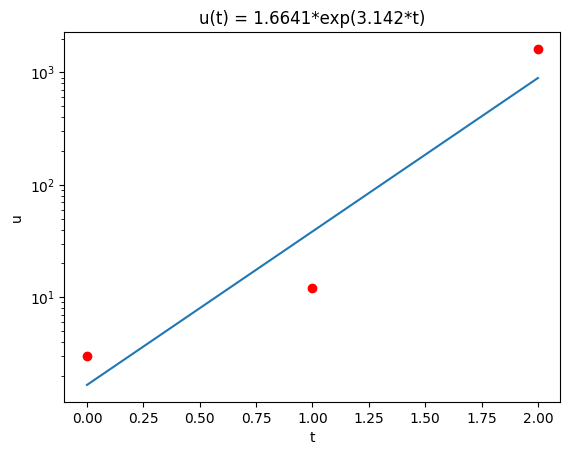
\includegraphics[width=\textwidth,height=0.4\textheight]{NUM1_HW005/output.png}}}
\caption{book}
\end{figure}

\end{document}
